\section{ATMS Response Data}
%===========================

\subsection{Specified and measured responses}
%--------------------------------------------
The NPP ATMS specified central frequencies, sideband offsets and channel bandwidths, taken from table 9 of the CrIS EDR ATBD\cite{CrIS_EDR_ATBD}, are shown in table \ref{tab:atms_fo_sb_and_df}. Also shown are measured bandwidths taken from table 12-1 of the ATMS PFM Calibration Data Book\cite{ATMS_PFM_CalLog}. No measurements of the central frequencies are readily available \footnote{These values may be available in other ATMS reports, particularly: RE-13680 K/Ka Band Receiver Shelf Verification Report, RE-13658 W Band Receiver Shelf Verification Report, RE-13741 V Band Receiver Shelf Verification Report, and RE-13802 G Band Receiver Shelf Verification Report.}.

\begin{table}[htp]
  \centering
  \begin{tabular}{c c c c c c}
    \hline
                     & \textbf{Central}         & \textbf{Sideband 1}   & \textbf{Sideband 2}   & \textbf{Specified}       & \textbf{Measured} \\
                     & \textbf{Frequency}\up{a} & \textbf{Offset}\up{a} & \textbf{Offset}\up{a} & \textbf{Bandwidth}\up{a} & \textbf{Bandwidth}\up{b} \\
    \textbf{Channel} & \bfrequency{0}           & \bsideband{1}         & \bsideband{2}         & \bdeltaf                 & \bdeltaf      \\
                     & (GHz)                    & (GHz)                 & (GHz)                 & (GHz)                    & (GHz)         \\
    \hline\hline
            1        &  23.800000  & -      & -      & 0.27   & 0.258         \\
            2        &  31.400000  & -      & -      & 0.18   & 0.172         \\
            3        &  50.300000  & -      & -      & 0.18   & 0.173         \\
            4        &  51.760000  & -      & -      & 0.40   & 0.381         \\
            5        &  52.800000  & -      & -      & 0.40   & 0.366         \\
            6        &  53.596000  & 0.115  & -      & 0.17   & 0.1587,0.1648\up{c} \\
            7        &  54.400000  & -      & -      & 0.40   & 0.387         \\
            8        &  54.940000  & -      & -      & 0.40   & 0.387         \\
            9        &  55.500000  & -      & -      & 0.33   & 0.317         \\
           10        &  57.290344  & -      & -      & 0.33   & 0.151         \\
           11        &  57.290344  & 0.217  & -      & 0.078  & 0.0763        \\
           12        &  57.290344  & 0.3222 & 0.048  & 0.036  & 0.0351        \\
           13        &  57.290344  & 0.3222 & 0.022  & 0.016  & 0.01547       \\
           14        &  57.290344  & 0.3222 & 0.010  & 0.008  & 0.0078,0.0079\up{c} \\
           15        &  57.290344  & 0.3222 & 0.0045 & 0.003  & 0.0029        \\
           16        &  88.200000  & -      & -      & 2.0    & 1.9282        \\
           17        & 165.500000  & -      & -      & 3.0    & 1.1251        \\
           18        & 183.310000  & 7.0    & -      & 2.0    & 1.9302        \\
           19        & 183.310000  & 4.5    & -      & 2.0    & 1.9519        \\
           20        & 183.310000  & 3.0    & -      & 1.0    & 0.9799        \\
           21        & 183.310000  & 1.8    & -      & 1.0    & 0.9823        \\
           22        & 183.310000  & 1.0    & -      & 0.5    & 0.4940        \\
    \hline
  \end{tabular}
  \caption{Central, sideband offset, and bandwidth frequencies for ATMS. \superscript{a}Data from table 9 of ref.\cite{CrIS_EDR_ATBD}. \superscript{b}Data from table 12-1 of ref.\cite{ATMS_PFM_CalLog}. \superscript{c}Different lower and upper sideband widths reported. }
  \label{tab:atms_fo_sb_and_df}
\end{table}

In addition to the usual frequency parameters, the ATMS PFM Calibration Data Book\cite{ATMS_PFM_CalLog} contains tables (12-2a to 12-2d) of the digitised filter responses (hereafter referred to as the spectral response functions, or SRFs). Apart from channels 1 and 2, these digitised SRFs are at the intermediate frequencies (IF) at which the measurements were made, not at the actual on-orbit channel frequencies. So, these IF SRFs need to be processed so as to represent the SRFs at the frequencies corresponding to the on-orbit channel radiance measurements. The procedures used to do this for the ``Table 12'' IF SRF are shown schemtatically in figure \ref{fig:r_and_s}. Two operations are performed: translation and reflection; how they are carried out depends on the ATMS channel:

\begin{figure}[htp]
  \centering
  \input{graphics/schematics/r_and_s.pstex_t}
  \caption{Schematic illustration of how the ATMS responses, measured at intermediate frequencies, were processed to SRFs at the measurement frequencies. \textbf{(a)} Single passband channels (3-5, 7-10, 16, 17). \textbf{(b)} Double passband channels (11, 18-22). \textbf{(c)} Quadruple passband channels (12-15). \textbf{(d)} Channel 6.}
  \label{fig:r_and_s}
\end{figure}

\begin{description}
  \item[Single Passband Channels, fig.\ref{fig:r_and_s}(a).] Channels 3-5,7-10,16,17. The measured IF SRFs are simply translated to the channel central frequency, $f_0$. The value of the IF central frequency, $f_{i,0}$, is obtained from the first moment of the SRF.
  \item[Double Sideband Channels, fig.\ref{fig:r_and_s}(b).] Channels 11, 18-22. Here a single measured IF sideband is reflected about 0GHz (corresponding to $f_{i,0}$ in this case) and the two sidebands are then translated to the channel central frequency, $f_0$.
  \item[Quadruple Sideband Channels, fig.\ref{fig:r_and_s}(c).] Channels 12-15. In this case two non-contiguous sidebands are reflected about 0GHz (again, corresponding to $f_{i,0}$) and all four sidebands are then translated to the channel central frequency. 
  \item[Channel 6, fig.\ref{fig:r_and_s}(d).] This channel is mentioned separately since, while it is a double sideband channel, unlike the other double sideband channels the IF SRF data contains the contiguous measurement of both sidebands. Thus only translation is applied to the IR SRF. As with the single passband channels, the IF central frequency is the first moment of the SRF. Note that this leads to a different bandwidth for the two sidebands; a situation one doesn't get for for the typical case in fig. \ref{fig:r_and_s}(b). It does beg the question as to why the same procedure wasn't performed for the other multi-band channels.
\end{description}

A selection of four channels from the Table 12 ATMS SRF data, compared to the boxcar reponse, are shown in figure \ref{fig:srf_selection}. All of the channel SRF are shown in appendix \ref{app:srf}. Two channels were selected for display in figure \ref{fig:srf_selection} to highlight their significant difference from the boxcar response: channel 10 (fig.\ref{fig:srf_selection}(b)) because the spec. bandwidth is quite different from that measured by about a factor of two\footnote{Channel 17 suffers similarly; see figure \ref{fig:atms_npp.ch17.srf}}; and channel 19 (fig.\ref{fig:srf_selection}(d)) because, while the measured data does cover the specified bandwidth, the in-band SRF magnitudes appear to decrease anomalously.

\begin{figure}[htp]
  \centering
  \begin{tabular}{c c}
    \textsf{\textbf{(a)} Channel 6} &
    \textsf{\textbf{(b)} Channel 10} \\
    \includegraphics[scale=0.5]{graphics/srf/atms_npp.ch6.srf.eps} &
    \includegraphics[scale=0.5]{graphics/srf/atms_npp.ch10.srf.eps} \\\\

    \textsf{\textbf{(c)} Channel 11} &
    \textsf{\textbf{(d)} Channel 19} \\
    \includegraphics[scale=0.5]{graphics/srf/atms_npp.ch11.srf.eps} &
    \includegraphics[scale=0.5]{graphics/srf/atms_npp.ch19.srf.eps}
  \end{tabular}
  \caption{Selection of NPP ATMS Table 12 SRF data from reference \cite{ATMS_PFM_CalLog} with the corresponding boxcar response based on table \ref{tab:atms_fo_sb_and_df} data.}
  \label{fig:srf_selection}
\end{figure}


\subsection{Additional Digitised Responses}
%------------------------------------------
After a recent SOAT meeting\footnote{Sounding Operational Algorithm Team (SOAT) Meeting, CrIS/ATMS Cal/Val Team, Integrated Program Office, Silver Spring, Maryland, USA, 20-21 May 2009} where the NPP ATMS Table 12 SRF data was discussed, two of us (Chidester, SDL; and DeAmici, NGAS) separately digitised the graphical SRFs displayed in the ATMS PFM Calibration Data Book\cite{ATMS_PFM_CalLog}. The SDL dataset consisted of channels 1, 12, 13, 14, and 15; and the NGAS dataset consisted of channels 4, 5, 9, 13, and 14. These digitised SRFs, along with the corresponding boxcar and Table 12 SRFs, are shown in figures \ref{fig:sp_digitised_srfs} (single passband channels) and \ref{fig:qp_digitised_srfs} (quadruple passband channels).

\begin{figure}[htp]
  \centering
  \begin{tabular}{c c}
    \textsf{\textbf{(a)} Channel 1} &
    \textsf{\textbf{(b)} Channel 4} \\
    \includegraphics[scale=0.5]{graphics/srf/atms_npp.ch1.srf.eps} &
    \includegraphics[scale=0.5]{graphics/srf/atms_npp.ch4.srf.eps} \\\\

    \textsf{\textbf{(c)} Channel 5} &
    \textsf{\textbf{(d)} Channel 9} \\
    \includegraphics[scale=0.5]{graphics/srf/atms_npp.ch5.srf.eps} &
    \includegraphics[scale=0.5]{graphics/srf/atms_npp.ch9.srf.eps}
  \end{tabular}
  % the hand-crafted legend
  \setlength{\unitlength}{1cm}
  \begin{picture}(2.0,2.0)
    \thicklines
    \color{blue}
    \put(0.0,0.2 ){\line(1,0){1}}
    \put(1.1,0.05){\sffamily NGAS}
    \color{green}
    \put(0.0,0.7 ){\line(1,0){1}}
    \put(1.1,0.55){\sffamily SDL}
    \color{red}
    \put(0.0,1.2 ){\line(1,0){1}}
    \put(1.1,1.05){\sffamily Table 12}
    \color{black}
    \put(0.0,1.7 ){\line(1,0){1}}
    \put(1.1,1.55){\sffamily Boxcar}
  \end{picture}
  \caption{Single passband SDL and NGAS digitised NPP ATMS SRFs from reference \cite{ATMS_PFM_CalLog} with the corresponding boxcar and Table 12 response}
  \label{fig:sp_digitised_srfs}
\end{figure}

For the single passband channels shown in figure \ref{fig:sp_digitised_srfs}, the SDL channel 1 digitisation of fig.\ref{fig:sp_digitised_srfs}(a) appears to be most like the Table 12 representation. For the NGAS digitisations, figs.\ref{fig:sp_digitised_srfs}(b)-(d), the outstanding feature is how very different the digitised data is from the Table 12 data. Lest readers think the digitisation procedures somehow went awry, they are referred to Appendix \ref{app:srf} -- in particular figures \ref{fig:atms_npp.ch1.srf}, \ref{fig:atms_npp.ch4.srf}, \ref{fig:atms_npp.ch5.srf}, and \ref{fig:atms_npp.ch9.srf} -- where the plots shown in \ref{fig:sp_digitised_srfs} are replicated at a larger size, but also with the corresponding filter response taken from the ATMS PFM Calibration Data Book \cite{ATMS_PFM_CalLog}. Comparison of these plots clearly show that the SDL and NGAS digitisations are more respresentative of the measurements displayed in \cite{ATMS_PFM_CalLog}.

\begin{figure}[htp]
  \centering
  \begin{tabular}{c c}
    \textsf{\textbf{(a)} Channel 12} &
    \textsf{\textbf{(b)} Channel 13} \\
    \includegraphics[scale=0.5]{graphics/srf/atms_npp.ch12.srf.eps} &
    \includegraphics[scale=0.5]{graphics/srf/atms_npp.ch13.srf.eps} \\\\

    \textsf{\textbf{(c)} Channel 14} &
    \textsf{\textbf{(d)} Channel 15} \\
    \includegraphics[scale=0.5]{graphics/srf/atms_npp.ch14.srf.eps} &
    \includegraphics[scale=0.5]{graphics/srf/atms_npp.ch15.srf.eps}
  \end{tabular}
  % the hand-crafted legend
  \setlength{\unitlength}{1cm}
  \begin{picture}(2.0,2.0)
    \thicklines
    \color{blue}
    \put(0.0,0.2 ){\line(1,0){1}}
    \put(1.1,0.05){\sffamily NGAS}
    \color{green}
    \put(0.0,0.7 ){\line(1,0){1}}
    \put(1.1,0.55){\sffamily SDL}
    \color{red}
    \put(0.0,1.2 ){\line(1,0){1}}
    \put(1.1,1.05){\sffamily Table 12}
    \color{black}
    \put(0.0,1.7 ){\line(1,0){1}}
    \put(1.1,1.55){\sffamily Boxcar}
  \end{picture}
  \caption{Quadruple passband SDL and NGAS digitised NPP ATMS SRFs from reference \cite{ATMS_PFM_CalLog} with the corresponding boxcar and Table 12 response}
  \label{fig:qp_digitised_srfs}
\end{figure}

Similarly, for the quadruple passband channels shown in figure \ref{fig:qp_digitised_srfs}, the SDL and NGAS digitisations are quite different from the Table 12 data. Of particular interest is the difference in relative magnitudes between the ``inner'' (\#2 and \#3) and ``outer'' (\#1 and \#4) bands for channels 13 and 14 in figs.\ref{fig:qp_digitised_srfs}(b) and (c). Comparison of the digitised data with that displayed in the ATMS PFM Calibration Data Book \cite{ATMS_PFM_CalLog} -- see figures \ref{fig:atms_npp.ch12.srf}, \ref{fig:atms_npp.ch13.srf}, \ref{fig:atms_npp.ch14.srf}, and \ref{fig:atms_npp.ch14.srf} -- again shows the SDL and NGAS digitisation to be more respresentative of the filter responses, in both shape and relative magnitude, than the Table 12 data. It should be pointed out that the vertical excursions for the relative response plots are more pronounced than for those where the y-axis is signal loss with units of decibels.
 

